% Úvod
%%%%%%%%%%%%%%%%%%%%%%%%%%%%%%%%%%%%%%%%%%%%%%%%%%%%%%%%%%%%%%%%%%%%%%%%%%%%%%%%%%%%%%%%%%%%%%
\section{Úvod}
Program MemSkel (\textbf{Mem}brane \textbf{Skel}etonization) je určen pro segmentaci buněčné stěny. Jedná se o~interatkivní metodu segmentace obrazu, která ke svému běhu potřebuje alespoň jednu výchozí pozici v~obraze. Tu uživatel do obrazu zadá pomocí myši. Takto označené body (pixely) se nazývají seedy (z~anglického výrazu \textit{seed points}). Výsledek segmentace je možný manuálně upravit nástrojem guma či přidáním dalších seedů. Jakmile je uživatel s~výsledkem spokojen, je možné spustit skeletonizaci, která najde střednici segmentované membrány. Je nutné, aby byl výsledek segmentace uzavřenou oblastí, jinak proces skeletonizace selže viz níže. Výsledný skelet je možné aproximovat pomocí b-spliny s~proměnnou mírou vyhlazení.

\begin{figure}[htb]
    \centering
    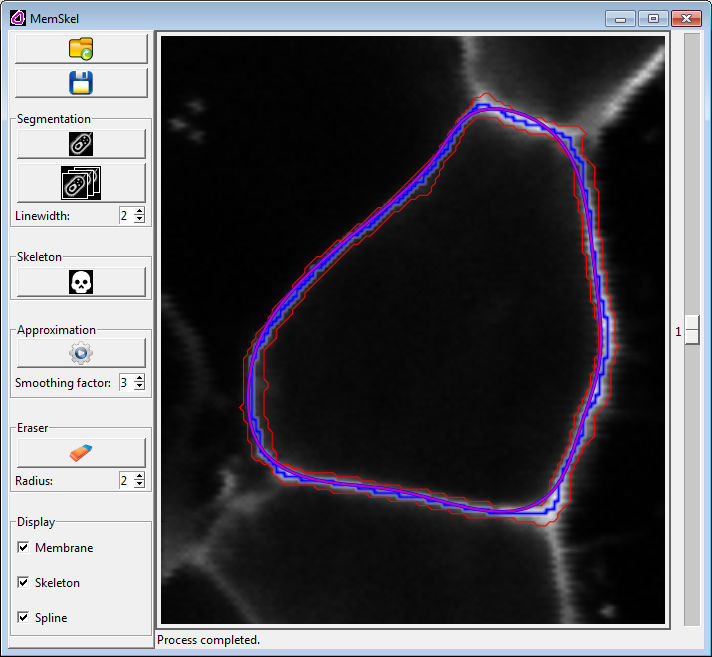
\includegraphics[width = .7\linewidth]{gui.png}
    \caption{Hlavní okno programu.}
    \label{fig:gui}
\end{figure}

% Grafické uživatelské rozhraní
%%%%%%%%%%%%%%%%%%%%%%%%%%%%%%%%%%%%%%%%%%%%%%%%%%%%%%%%%%%%%%%%%%%%%%%%%%%%%%%%%%%%%%%%%%%%%%
\section{Grafické uživatelské rozhraní} \label{sec:stEd}
Aplikace je rozdělena do dvou hlavních částí: nástrojová lišta, vizualizace. V~následující části jsou popsány všechny hlavní prvky grafického uživatelského rozhraní, které jsou očíslovány na obr. \ref{fig:gui_labeled}.

\begin{figure}[htb]
    \centering
    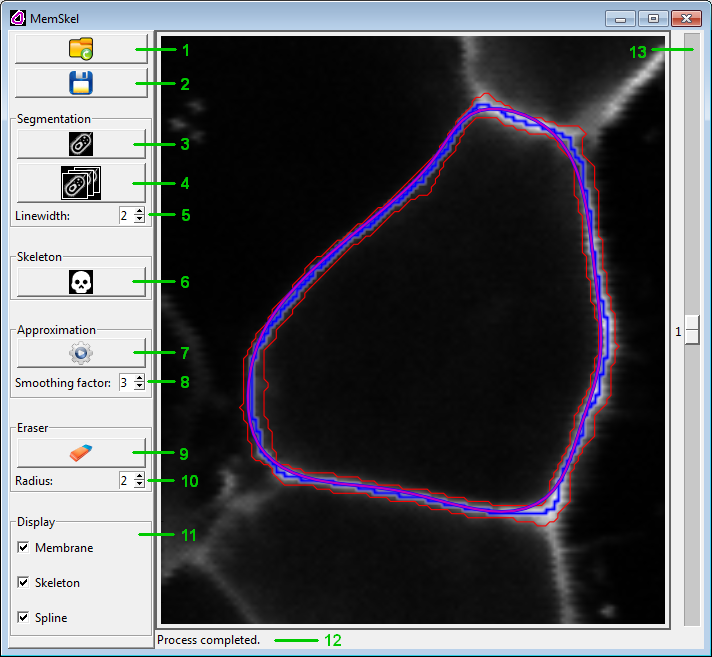
\includegraphics[width = .7\textwidth]{gui_labeled.png}
    \caption{Hlavní okno programu s~očíslovanými částmi.}
    \label{fig:gui_labeled}
\end{figure}

V~následujícím výčtu je uveden krátký popis jednotlivých částí:
\begin{enumerate}
    \item Otevřít soubor \ldots otevře dialog pro načtení dat ze souboru.
	\item Uložit \ldots otevře dialog pro uložení výsledků práce.
	\item Segmentace jednoho snímku \ldots v~případě dat obsahujících více než jeden snímek (frame, page), provede segmentaci pouze aktuálního snímku.
	\item Segmentace stacku \ldots v~případě dat obsahujících více než jeden snímek (frame, page), provede segmentaci celého stacku (všech framů).
	\item Linewidth \ldots spinbox pro změnu šířky čáry, používané při označování membrány.
	\item Skeletonization \ldots spustí skeletonizaci masky membrány a vypočítá její střednici.
	\item Approximation \ldots aproximuje střednici masky membrány s mírou vyhlaení danou následujícím parametrem.
	\item Smoothing factor \ldots spinbox pro určení míry s jakou bude aproximována střednice masky membrány.
	\item Eraser \ldots spustí nástroj guma pro mazání masky membrány.
	\item Radius \ldots spinbox pro změnu velikosti gumy.
	\item Display \ldots checkboxy pro zapnutí/vypnutí vizualizace příslušných prvků.
	\item Status bar \ldots zobrazuje informace o~běhu programu.
	\item Slider \ldots umožňuje změnu snímku načtených dat.
\end{enumerate}


% Používání editoru
%%%%%%%%%%%%%%%%%%%%%%%%%%%%%%%%%%%%%%%%%%%%%%%%%%%%%%%%%%%%%%%%%%%%%%%%%%%%%%%%%%%%%%%%%%%%%%
\section{Používání aplikace}
Následující část bude obsahovat odkazy na jednotlivé komponenty grafického rozhraní, které jsou očíslovány na obr. \ref{fig:gui_labeled}. Odkazy budou ve formě kroužku s~příslušným číslem uvnitř, např. odkaz na tlačítko pro otevření souboru má tvar \circled{1}.

%%%%%%%%%%%%%%%%%%%%%%%%%%%%%%%%%%%%%%%%%%%%%%%%%%%%%%%%%%%%%%%%%%%%%%%%%%%%%%%%%%%%%%%%%%%%%%
\subsection{Spuštění a ukončení}
Editor se spouští souborem \textit{memSkel\_main.exe } a ukončuje se kliknutím na červený křížek v~pravém horním rohu okna.

%%%%%%%%%%%%%%%%%%%%%%%%%%%%%%%%%%%%%%%%%%%%%%%%%%%%%%%%%%%%%%%%%%%%%%%%%%%%%%%%%%%%%%%%%%%%%%
\subsection{Načtení dat}
Stiskem tlačítka \circled{1} se otevře dialog pro otevření souboru. Předpokládá se, že vstupní data budou ve formátu TIFF. Je nutné zajistit, aby byl formát kompletní, především aby obsahoval metainformace o~velikosti jednotlivých snímků. Pokud bude problem s~načtením dat, \uv{přeuložení} obrázku v~prohlížeči/editoru obrázků může pomoci. Např. program \textit{IrfanView} při možnosti \textit{Save as...} metainformace vytvoří. Jinou možností, která v~tomto případě může pomoci, je uložit data jako 8-bitová (na výstup programu tato změna nemá vliv).

Jakmile jsou data úspěšně načtena, zobrazí se v~editoru.

%%%%%%%%%%%%%%%%%%%%%%%%%%%%%%%%%%%%%%%%%%%%%%%%%%%%%%%%%%%%%%%%%%%%%%%%%%%%%%%%%%%%%%%%%%%%%%
\subsection{Segmentace membrány}
Jak již bylo řečeno, pro segmentaci membrány potřebuje algoritmus znát alespoň jeden výchozí bod (seed). Po stisku tlačítka \circled{3} resp. \circled{4} se spustí editační mód, ve kterém uživatel tahem myši (levé tlačítko stisknuté) označí seedy. Stiskem tlačítka enter se spustí se výpočetní algoritmus, po jehož doběhnutí má uživatel možnost podle potřeby domalovat další seedy a stiskem enteru spustit algoritmus znovu.

Po ukončení označování a stisku enteru, tzn. algoritmus doběhl a nebyly přidány další seedy, se editační mód ukončí. Poté je možné výsledek upravit pomocí nástroje guma, viz níže.

Během editačního módu je možné měnit šířku čáry pomocí spinboxu \circled{5} nebo kolečkem myši.

Stiskem tlačítka \circled{4} se spustí segmentace celého stacku, tzn. všech snímků. V~tomto případě začne algoritmus po ukončení segmentace aktuálního snímku (včetně možnosti přidání seedů) výsledek \uv{rozšiřovat} do dalších snímků. K~tomu je zapotřebí již skeleton prvního snímku, jeho výpočet se tedy spustí automaticky. Editace masky membrány je možná po doběhnutí algoritmu do konce.

%%%%%%%%%%%%%%%%%%%%%%%%%%%%%%%%%%%%%%%%%%%%%%%%%%%%%%%%%%%%%%%%%%%%%%%%%%%%%%%%%%%%%%%%%%%%%%
\subsection{Nástroj guma}
Pomocí tohoto nástroje (tlačítko \circled{9} nebo tlačítko \textit{e}) je možné editovat binární masku membrány. Aktivita tohoto nástroje je indikována modrým kolečkem kolem kurzoru, jehož velikost koresponduje s~velikostí okolí, které je editováno. Poloměr nástroje guma je možný měnit pomocí spinboxu \circled{10} nebo kolečkem myši, pokud je nástroj aktivní. Po stisku levého tlačítka myši se spustí mazací režim, který vymaže všechny pixely v~masce membrány, které jsou lokalizovány v~oblasti dané kolečkem kolem kurzoru. Samozřejmostí je i možnost tažení myši. Aktivace mazacího režimu je indikována zbarvením tohoto kolečka do červena, viz obr. \ref{fig:eraser}.

\begin{figure}[htb]
	\centering
	\subfloat[]{\label{fig:eraserA}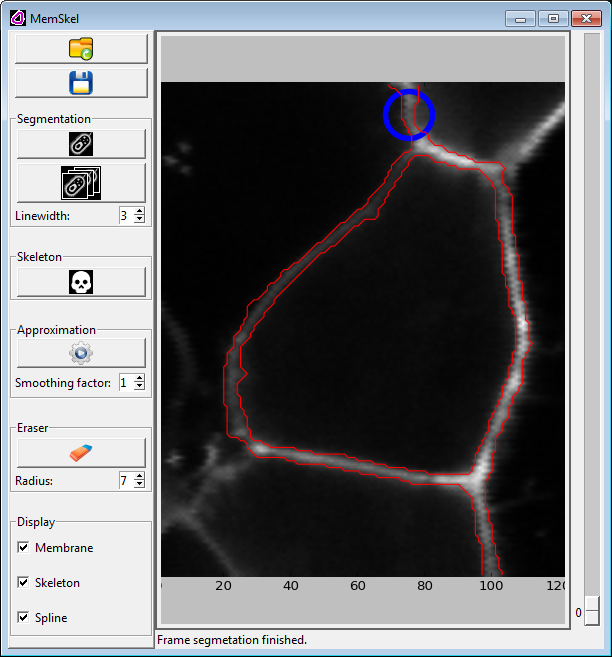
\includegraphics[width=0.45\textwidth]{eraser3.png}}
	\hskip 0.1cm
	\subfloat[]{\label{fig:eraserB}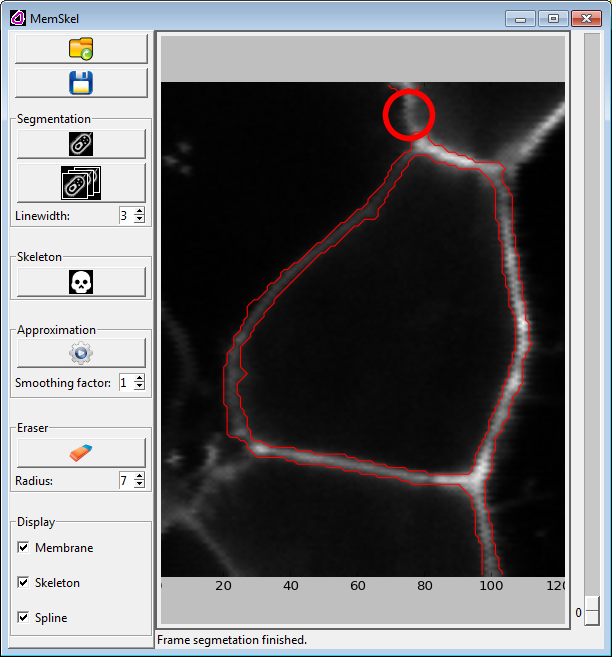
\includegraphics[width=0.45\textwidth]{eraser4.png}}
	\caption{Demonstrace nástroje guma. Na obr. \ref{fig:eraserA} je znázorněn stav, kdy je nástroj guma spuštěn, obr. \ref{fig:eraserB} pak znázorňuje stav při stisku levého tlačítka myši.}
	\label{fig:eraser}
\end{figure}

%%%%%%%%%%%%%%%%%%%%%%%%%%%%%%%%%%%%%%%%%%%%%%%%%%%%%%%%%%%%%%%%%%%%%%%%%%%%%%%%%%%%%%%%%%%%%%
\subsection{Skeletonizace}
Jakmile je určena maska membrány, je dalším krokem určení její střednice (středové osy). Toho je docíleno stiskem tlačítka \circled{6}. Pro správnou funkčnost je nutné, aby byla membrána uzavřená, jinak nebude algoritmus fungovat, viz obr. \ref{fig:skel}. 

\begin{figure}[htb]
	\centering
	\subfloat[]{\label{fig:skelA1}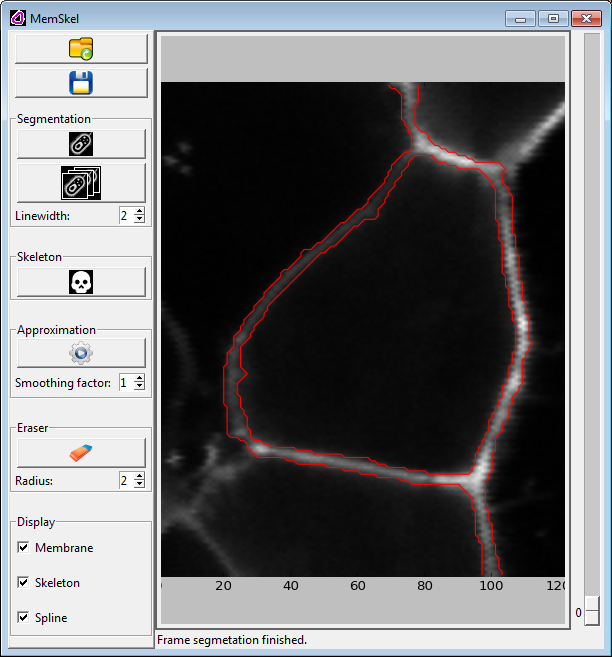
\includegraphics[width=0.45\textwidth]{skelA1.png}}
	\hskip 0.1cm
	\subfloat[]{\label{fig:skelA2}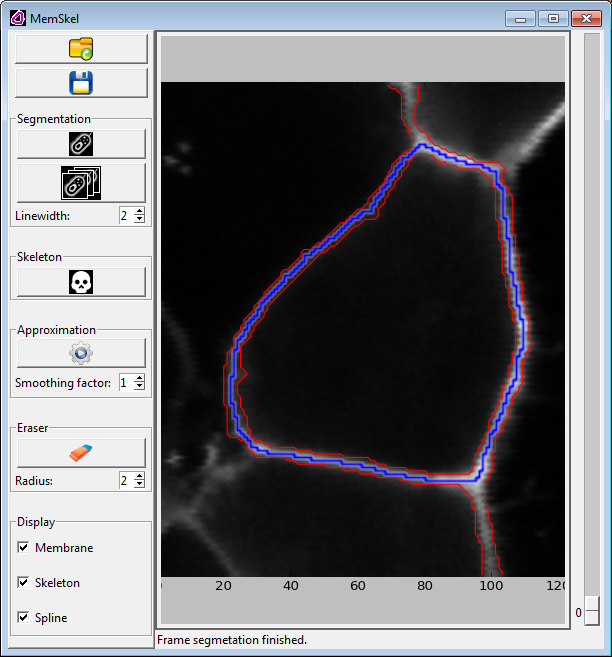
\includegraphics[width=0.45\textwidth]{skelA2.png}}
	\\
	\subfloat[]{\label{fig:skelB1}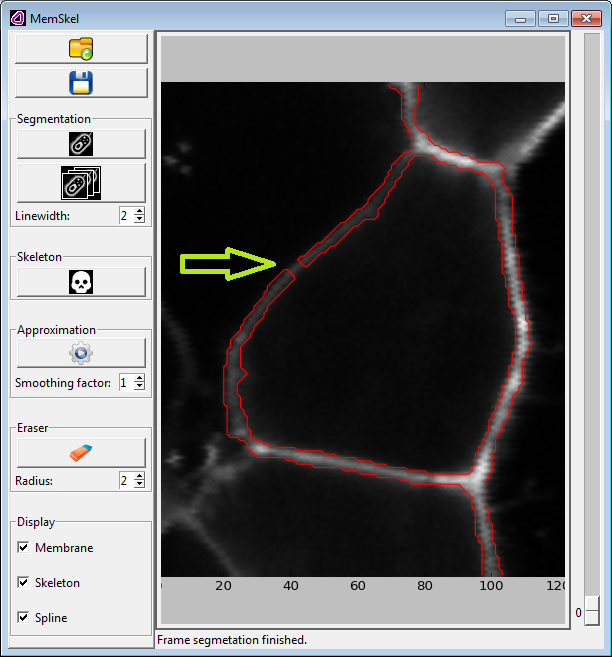
\includegraphics[width=0.45\textwidth]{skelB1.png}}
	\hskip 0.1cm
	\subfloat[]{\label{fig:skelB2}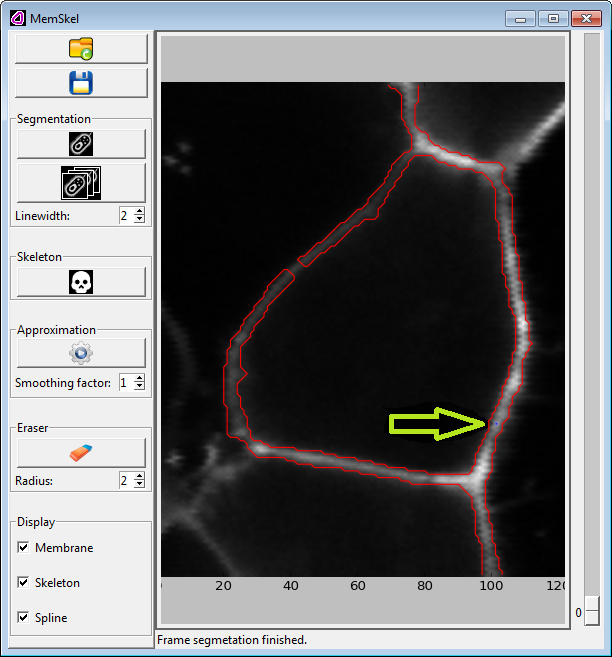
\includegraphics[width=0.45\textwidth]{skelB2.png}}
	\caption{Demonstrace použití nástroje pro určení střednice. Obr. \ref{fig:skelA1} je znázorněna správně segmentovaná membrána a příslušná střednice je na obr. \ref{fig:skelA2}. V~případě špatně segmentované membrány viz \ref{fig:skelB1}, selže i výpočet střednice viz \ref{fig:skelB2}.}
	\label{fig:skel}
\end{figure}

%%%%%%%%%%%%%%%%%%%%%%%%%%%%%%%%%%%%%%%%%%%%%%%%%%%%%%%%%%%%%%%%%%%%%%%%%%%%%%%%%%%%%%%%%%%%%%
\subsection{Aproximace}
Po určení střednice je možné provést její aproximaci pomocí b-spliny stiskem tlačítka \circled{7}. Současně je možné měnit i míru vyhlazení pomocí spinboxu \circled{8}. Demonstrace tohoto nástroje je zobrazena na následujícím obrázku \ref{fig:spline}.

\begin{figure}[htb]
	\centering
	\subfloat[]{\label{fig:spline1}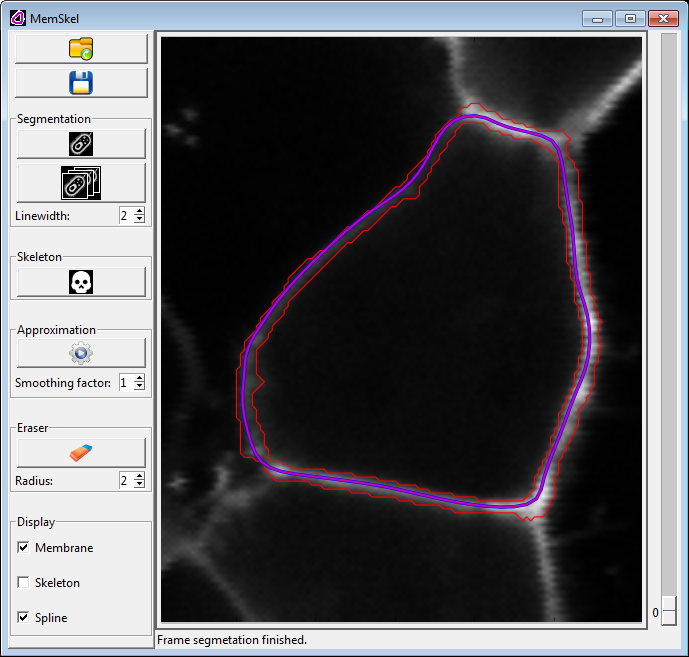
\includegraphics[width=0.45\textwidth]{app1.png}}
	\hskip 0.1cm
	\subfloat[]{\label{fig:spline2}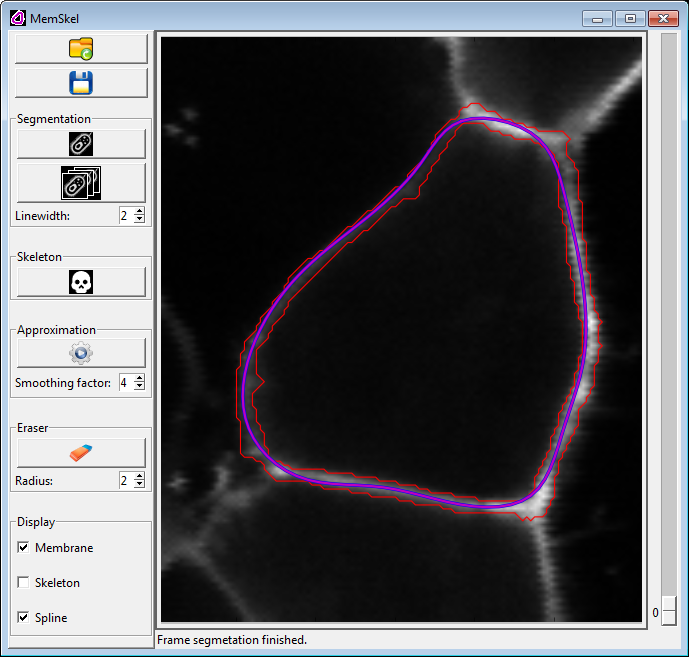
\includegraphics[width=0.45\textwidth]{app4.png}}
	\\
	\subfloat[]{\label{fig:spline3}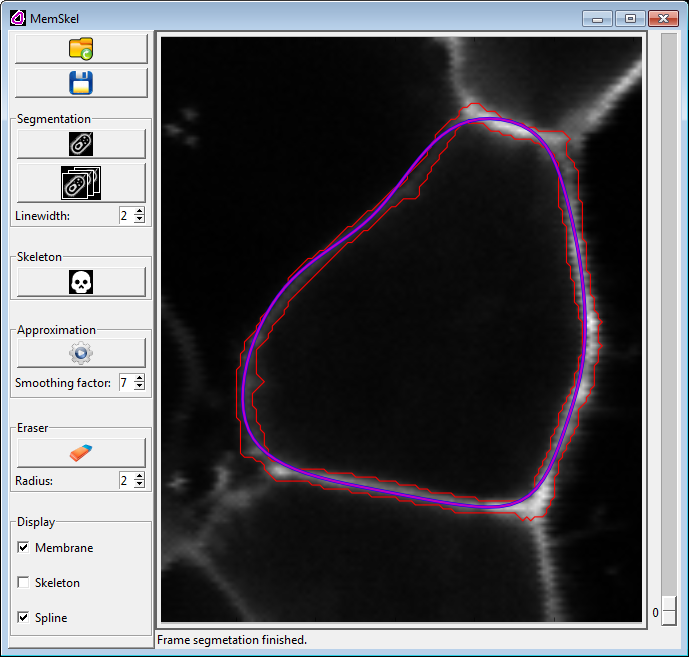
\includegraphics[width=0.45\textwidth]{app7.png}}
	\hskip 0.1cm
	\subfloat[]{\label{fig:spline4}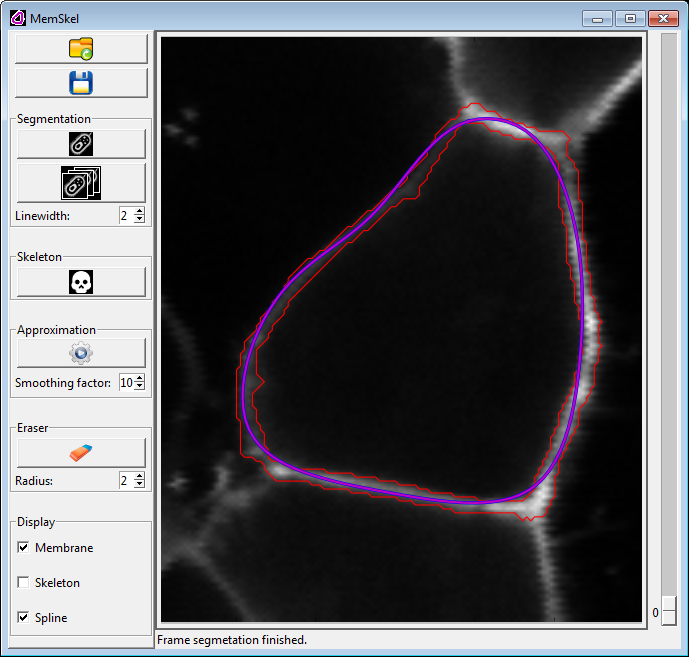
\includegraphics[width=0.45\textwidth]{app10.png}}
	\caption{Demonstrace aproximace splinou a různých stupňu vyhlazení: faktor = 1 ... \ref{fig:spline1}, faktor = 4 ... \ref{fig:spline2}, faktor = 7 ... \ref{fig:spline3} a faktor = 10 ... \ref{fig:spline4}.}
	\label{fig:spline}
\end{figure}

%%%%%%%%%%%%%%%%%%%%%%%%%%%%%%%%%%%%%%%%%%%%%%%%%%%%%%%%%%%%%%%%%%%%%%%%%%%%%%%%%%%%%%%%%%%%%%
\subsection{Uložení výsledků}
Po dokončení práce je možné uložit výsledky pomocí tlačítka \circled{2}. Program vytvoří dva soubory:
\begin{enumerate}
	\item binární obrázek představující výslednou masku membrány,
	\item textový souboru popisující aproximační splinu (uzly).
\end{enumerate}

% Ostatní
%%%%%%%%%%%%%%%%%%%%%%%%%%%%%%%%%%%%%%%%%%%%%%%%%%%%%%%%%%%%%%%%%%%%%%%%%%%%%%%%%%%%%%%%%%%%%%
\section{Ostatní}

\subsection{Status bar}
Ve status baru \circled{12}, se zobrazují hlavní informace o~činnosti editoru. Mezi ně patří informace o~úspěšném/neúspěšném načtení dat, průběhu algoritmů, úspěšném/neúspěšném uložení výsledků apod. Při segmentaci více-snímkových dat se v~pravé části zobrazí i tzv. progress bar, který udává procentuální stav výpočtu.

\subsection{Log file}
Při kritické chybě editoru, při níž dojde k~jeho ukončení, se objeví okno informující uživatele o~zápisu dané chyby do tzv. log souboru. Tento soubor má název \textit{memskel\_main.exe.log} a obsahuje bližší informaci o~místě v~programu, které vyvolalo pád editoru. Tento soubor je důležitý pro případné hlášení dané chyby vyvojářům.

%\subsection{Podporované OS}
%Editor je vytvořen na operačním systému Windows, současné podporované verze jsou Win 7 a Win XP. Editor funguje jak na 32-bitových tak i na 64-bitových operačních systémech.
% Ostatní
%%%%%%%%%%%%%%%%%%%%%%%%%%%%%%%%%%%%%%%%%%%%%%%%%%%%%%%%%%%%%%%%%%%%%%%%%%%%%%%%%%%%%%%%%%%%%%
\section{Spuštění programu ze zdrojových dat}
Tato kapitola popisuje postup instalace Pythonu a balíků, které jsou v programu využívány. Toho je zapotřebí v případě spouštění programu ze zdrojových dat.
\subsection{Potřebné balíky}
V této sekci jsou vyjmenovány všechny balíky, které program využívá a tudíž potřebuje ke svému běhu. Uvedena je i verze daných balíků.
\begin{itemize}
	\item Python 2.7.5
	\item numpy-MKL-1.7.1
	\item scipy-0.12.0
	\item matplotlib-1.1.1 (s novějšími verzemi program nefunguje - nezachytává klávesy), před instalací nutno nainstalovat následující podmiňující balíky:
		\begin{itemize}
			\item python-dateutil-1.5
			\item pytz-2013b
			\item pyparsing-1.5.7
		\end{itemize}
	\item pylibtiff-0.3.0.dev82
	\item Pillov-2.0.0
\end{itemize}

%------------------------------------------------------------------------------
\subsection{Pořadí instalace balíků}
Při samotné instalaci je zapotřebí dodržovat určité pořadí, ve kterém jsou balíky do Pythonu přidávány:
\begin{enumerate}
	\item python-2.7.5.msi \ldots instaluje samotný jazyk Python; v~tomto kroku nezáleží na tom, jestli se nainstaluje 32 nebo 64 bitová verze, je ale nutné další balíky volit ve stejné bitové verzi,
	\item numpy-MKL-1.7.1.win32-py2.7.exe \ldots výpočetní jádro pythonu, práce s vícerozměrnými poli apod,
	\item scipy-0.12.0.win32-py2.7.exe \ldots balík obsahující mmj. metody pro aproximaci,
	\item python-dateutil-1.5.win32-py2.7.exe \ldots prerekvizita pro balík matplotlib,
	\item pytz-2013b.win32-py2.7.exe \ldots prerekvizita pro balík matplotlib,
	\item pyparsing-1.5.7.win32-py2.7.exe \ldots prerekvizita pro balík matplotlib,
	\item matplotlib-1.1.1.win32-py2.7.exe \ldots vizualizace, novější verze balíku nefungují,
	\item pylibtiff-0.3.0.dev82.win32-py2.7.exe \ldots práce s obrázky typu TIFF,
	\item Pillow-2.0.0.win32-py2.7.exe \ldots práce s obrázky, načítání apod,
	\item setuptools-0.7.4.win32-py2.7.exe \ldots instalace balíků ze zdrojových kódů,
	\item pymorph-0.96 \ldots morfologické úpravy obrázku; instalace viz níže.
\end{enumerate}

Pro instalaci balíku \textit{pymorph} je nutné přidat python do systémové proměnné PATH. Může se stát, že nějaký instalační balík tak učiní automaticky - v takovém případě tento krok není nutný. Pro ověření je třeba spustit příkazovou řádku (command line), např. stiskem \textit{Win+R} a vepsáním \textit{cmd} do otevřeného okna viz obr. \ref{fig:run_cmd}. Vepsáním příkazu \textit{python --help} do spuštěné příkazové řádky by se měla zobrazit nápověda pro programovací jazyk viz obr. \ref{fig:cmd_python_help_OK}. Pokud se ale zobrazí okno viz obr. \ref{fig:cmd_python_help_KO}, znamená to, že je třeba python přidat do systémové proměnné. To lze jednoduše zařídit příkazem \textit{setx path "\%path\%;c:$\backslash$Python27"}, měla by se poté vypsat hláška potvrzující přidání, viz obr. \ref{fig:cmd_python_added}. Po restartování příkazové řádky by se po zopakování experimentu měla zobrazit hláška viz \ref{fig:cmd_python_help_OK}.

\begin{figure}[htb]
	\centering
	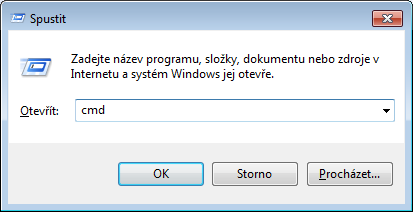
\includegraphics[width=0.4\textwidth]{spustit_cmd.png}
	\caption{Spuštění příkazové řádky.}
	\label{fig:run_cmd}
\end{figure}

\begin{figure}[htb]
	\centering
	\subfloat[Python zaveden v promenne PATH]{\label{fig:cmd_python_help_OK}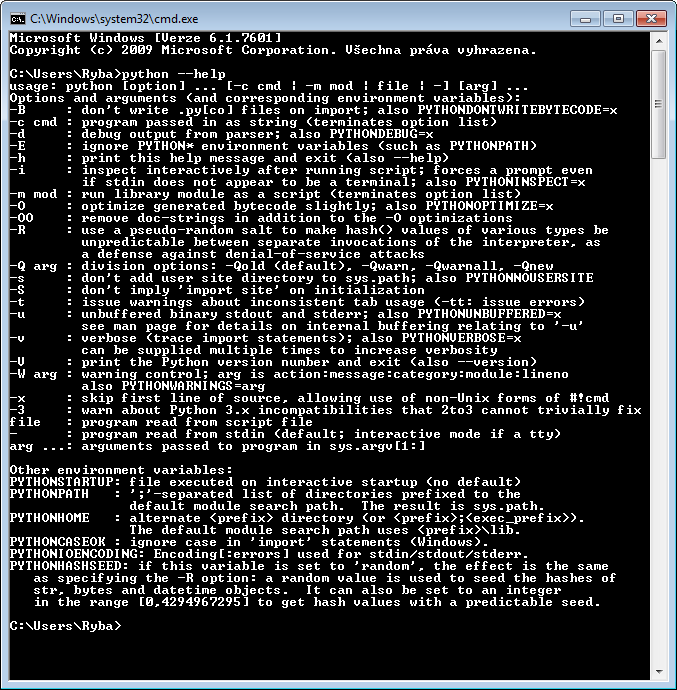
\includegraphics[width=0.45\textwidth]{cmd_python_help_OK.png}}
	\hskip 0.2cm
	\subfloat[Python nezaveden v promenne PATH]{\label{fig:cmd_python_help_KO}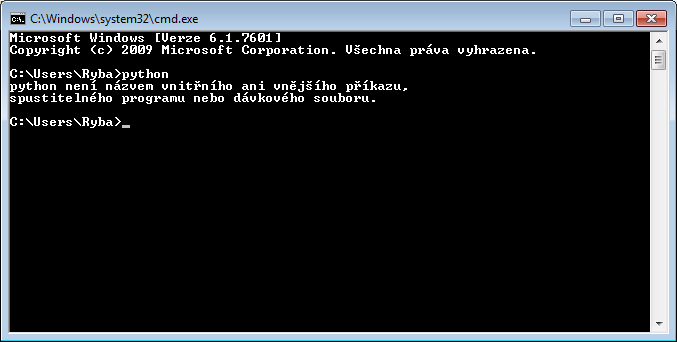
\includegraphics[width=0.45\textwidth]{cmd_python_help_KO.png}}
	\caption{Ověření zavedení pythonu v systémové proměnné.}
	\label{fig:cmd_python_help}
\end{figure}

\begin{figure}[htb]
	\centering
	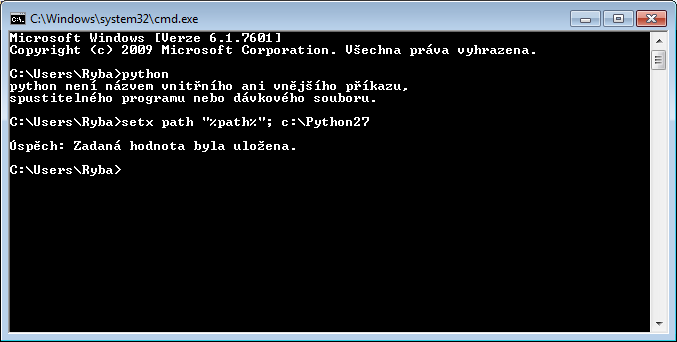
\includegraphics[width=0.4\textwidth]{cmd_python_added.png}
	\caption{Přidání pythonu do systémové proměnné.}
	\label{fig:cmd_python_added}
\end{figure}

Jakmile je přidána cesta do systémové proměnné, je možné nainstalovat balík \textit{pymorph} pomocí balíku \textit{setuptools}. Je nutné v~příkazové řádce přejít do adresáře \textit{pymorph-0.96} a instalaci spustit pomocí příkazu \textit{python setup.py install}. Pokud proběhne instalace správně, bude příkazová řádka vypadat podobně jako na obr. \ref{fig:cmd_pymorph}.

\begin{figure}[htb]
	\centering
	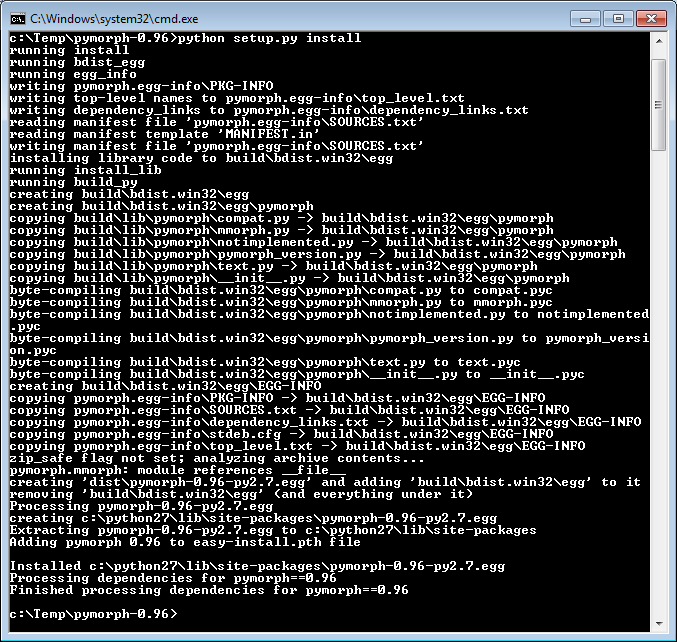
\includegraphics[width=0.4\textwidth]{cmd_pymorph.png}
	\caption{Instalace balíku \textit{pymorph}.}
	\label{fig:cmd_pymorph}
\end{figure}

%------------------------------------------------------------------------------
\subsection{Spuštění programu}
Jakmile je python přidán do systémové proměnné, je možné program MemSkel spustit spuštěním souboru \textit{memSkel\_main.py}, který se nachází přímo mezi zdrojovými daty. Eventuelně je možné spustit program z~příkazové řádky příkazem \textit{python memSkel\_main.py}, je třeba nacházet se v~adresáři, který daný soubor obsahuje, viz obr. \ref{fig:run}.

\begin{figure}[htb]
	\centering
	
\includegraphics[width=0.4\textwidth]{run.png}
	\caption{Spuštění programu MemSkel z~příkazové řádky.}
	\label{fig:run}
\end{figure}